\chapter{Modular formalism for stochastic~models}
\label{chap:rgspn}

In our current work we aim to propose an approach for the construction of stochastic models from engineering models without human intervention in order to evaluate automatically derived architecture proposals in design-space exploration by stochastic analysis.

The proposed transformation process should be flexible in the sense that---instead of basing our approach on a single engineering modeling language such as \textabbr{UML}~\citep{Rumbaugh04uml}, Sys\mixedabbr{ML}~\citep{Friedenthal16sysml}, \textabbr{AADL}~\citep{Feiler12aadl} or Palladio~\citep{Becker08palladio}---the creation of transformations for new architectural domain-specific languages (\textAbbr{DSL}s) in new problem domains should be supported and should not demand additional specialized knowledge from the users. Therefore the formal models should be based on a stochastic formalism that has sufficient descriptive power to support engineering practice. In addition, compatibility of the derived models with existing stochastic verification tools should be ensured so that recent developments in formal methods may be leveraged for high-performance analysis. Hence reusing an existing formalism is dictated by both \circled{1}~ease of use and \circled{2}~portability.

Analysis tools separate the input formal model and the \emph{query} to be answered \todo*{cite}, which is usually a performance metric to be calculated or a logical requirement to be verified. Therefore, when stochastic models are automatically derived for design-space exploration, \circled{3}~the appropriate queries must also be generated. The queries, which may depend on the structure of the engineering model in the same way as the derived stochastic model, serve as the objective functions and constraints of the exploration strategy.

To achieve these three objectives, in this chapter we turn to stochastic modeling approaches with modules to propose a formalism for the \emph{modules} (or \emph{fragments}) of the stochastic model corresponding to the analyzed aspects of the engineering model. The transformation, which is discussed in \cref{chap:transform}, will instantiate the modules specified by the user to automatically derive the analysis model.

After briefly reviewing related work, we describe our proposed formalism based on modular Petri nets, an extension of the \textabbr{ISO}/\textabbr{IEC}~15909-1:\citeyear{ISO1590912004} standard on High-level Petri nets with a formally defined module concept~\citep{Kindler09modular}.

Petri nets and their extension to stochastic modeling, generalized stochastic Petri nets (\textAbbr{GSPN}s) are a widely used formalism for the analysis of software and hardware systems~\citep{Murata89petri}. Various tools support \textAbbr{GSPN}s, such as \textabbr{SPNP}~\citep{Hirel00spnp}, \textabbr{SMART}~\citep{Ciardo06smart}, M\"obius~\citep{Courtney09mobius}, Great\mixedabbr{SPN}~\citep{Babar10greatspn} and Petri\-Dot\-Net~\citep{Voros17pdn}. Hence we believe most of the target audience of our transformation design-space exploration approach are familiar with them. In addition, to aid finding bugs in the analysis models and to contribute to the \circled{1}~ease of use, static typing, which was first proposed for modular high-level Petri nets by \citet{Kindler07modular}, is supported for both the stochastic model and queries.

Models are serialized in the \textabbr{ISO}/\textabbr{IEC}~15909-2:\citeyear{ISO1590922011} \textabbr{PNML} format for \circled{2}~compatibility with a wide variety of external tools.

In order to \circled{3} generate queries for the stochastic models, we follow \citet{Kindler01modular} and extend modular Petri nets with symbols corresponding to the stochastic properties of interest to encode the queries simultaneously with the structure of the analysis model.

\section{Related work: modular stochastic modeling}

In this section we briefly review some existing approaches for modular construction of logical and stochastic formal models, as well as for the specification of properties and metrics of interest over such models. For an overview on performance evaluation techniques for particular component-based software engineering languages, contrasting with our present work that aims to be generic in the engineering \textabbr{DSL}, we direct the interested reader to the survey by~\citet{Koziolek10review}.

We are especially interested in \emph{modular} formalisms that allow assembling structured models from modules (or fragments). While arbitrary combination of modules leads to high expressivity, it also restricts the opportunities for \emph{compositional} verification. On the other hand, a formalism is compositional if the properties of model can be verified recursively by verifying simpler properties of its constituent components. These models are often constructed using \emph{composition operators} that restrict arbitrary modularity in order to enforce property preservation. \todo{Cite!---V{\"o}ri said he has a good reference about this disctinction.}

We opt for modularity instead of compositionality to avoid restricting the model transformations that will automatically assemble the stochastic models according to an architectural \textabbr{DSL} instance. However, this means solution techniques will have to consider the assembled model in its entierty and cannot depend on preservation of the properties of the components.

\subsection{Modeling formalisms}

Continuous-time Markov chains (\textAbbr{CTMC}s) are common tools for the reliability and performability prediction of critical systems~(see e.g.~\cite{Reibman89markov}). However, instead of modeling with \textAbbr{CTMC}s directly, usually higher-level formalisms are used to obtain more compact models. The semantics of these models are defined in terms of \textAbbr{CTMC}s or related stochastic processes, such as Markov regenerative processes~\citep{Logothetis95mrm,Telek96mrm}. Usually the higher-level formalism belongs to one of these three classes:

\newpara \textbf{Queuing networks} (\textAbbr{QN}s) describe the routing of \emph{customers} or \emph{work items} between \emph{queues}. The times spent in queues are described by random variables. \todo{Should we cite a review about \textAbbr{QN}s?}

\newpara \textbf{Stochastic Petri nets} (\textAbbr{SPN}s) are Petri nets where transitions are equiped with expontentially distributed \emph{firing delays}. Generalized stochastic Petri nets (\textAbbr{GSPN}s), may contain transitions with either exponentially distributed delays and \emph{immediate} firing~\citep{Marsan84gspn}. Moreover, deterministic~\citep{Logothetis95mrm} and phase-type distributed~\citep{Longo13phasetype} delays may also be incorporated; however, this makes verification significantly more complicated. Another generalization is the stochastic activity network formalism, where arbitrary input and output gates are allowed~\citep{Sanders01san}.

\newpara \textbf{Stochastic process algebras} incorporate random timings into the denotational semantics of process calculi~\citep{Hermanns02algebra} while allowing compositional verification. However, composition is syntactically restricted to set of allowed process operators, such as parallel and sequential composition of two subprocesses. An example formalism of this class is the Performance Enhanced Process Algebra (\textabbr{PEPA}) defined by \citet{Hillston95pepa}.

\newpara Although all \textAbbr{CTMC}s can be expressed with any of these formalism classes, a significant advantage of higher-level models is the ability to expresses complicated behaviors of systems with small models. In this regard, \textAbbr{GSPN}s can express \textAbbr{QN}s without increasing model size~\citep{Vernon86comparison}. Comparison of Petri nets and process algebras is more difficult due to the vastly differing modeling styles~\citep{Donatelli95comparison}. The definable composition operators for Petri nets only conserve a limited set of properties; for a review we refer to Chapter~2 of the book by \citet{Hejiao12pppnpa}.

\todo*{Write about actual modular formalisms}

\subsection{Query specifications}

\todo*{Review modular query specification languages}

\section{Generalized stochastic Petri net modules}

In this section we propose the specification of modules for \textabbr{GSPN}s simultaneously with their reward measures and queries. When doing so, contradictions may arise in assembling the stochastic model from modules concerning the initial markings of places, the timings to transition firings and the definitions of the queries. In addition, care must be taken to avoid \emph{circularity} in the merged models and queries, i.e.~the structure of the model must not depend on the answers to the queries, as the state space and the \textabbr{CTMC} derived from the model is used in producing the answer. Hence circular dependence between the model and queries makes analysis impossible.

To address these challenges, we base our approach on modular Petri nets~\citep{Kindler01modular}, which define modules as a collection of \emph{symbols} (also referred to as \emph{nodes}) and the \emph{arcs} between them. Petri net places and transitions are represented as symbols. A symbol may either be \emph{concrete} symbol or a \emph{reference} to another symbol. \emph{Imports} of a module are references that are pointed to \emph{exports} of ther modules when the module is instantiated.

A module may only specify additional information about a concrete symbol, such as the initial marking of a concrete place or the rate of a timed transition. Thus there is a master-slave relationship between concrete and reference symbols, which avoids contradictions in assembled models. The specification of measures and queries is restricted analogously.

We incorporate three new symbol \emph{kinds} into modular Petri nets to construct modular \textabbr{GSPN}s. In addition, an \emph{expression language} is proposed to specify the values of both the stochastic attributes of the model elements, such as transition firing rates, and the performance measures and queries of interest. Circularity in models is avoided by an adapting strict typing to mark invalid dependencies as type errors. This approach was inspired by the work of~\citet{Kindler07modular} on strictly typed colored Petri net modules. We call the resulting formalism with extended symbols, expressions and typing \emph{reference generalized stochastic Petri nets} (\textabbr{RGSPN}).

To simplify presentation the separation of module interfaces and implementations, which enable information hiding for the design of modules, will be not considered. Moreover, the assembly of modules into a complete stochastic model is deferred to \cref{chap:transform}. The remainder of this chapter will focus on the structure and semantics of single \textabbr{RGSPN} modules and the \emph{inlining} of \textAbbr{RGSPN}s into \textAbbr{GSPN}s without references, which can be analyzed with existing tools. 

\subsection{Symbols and edges}

The \textabbr{RGSPN} formalism consists of symbols, and \emph{edges} between the symbols. The latter generalize Petri net arcs by also permitting reference assignments and collection memberships among the edges of the Petri net graph.

Each symbol has a \emph{kind}\todo{We should find a better term than \emph{kind}, as in the current implementation, this term is used in another (slightly related) sense for determining the appearance of symbols in textual and graphical concrete syntaxes.},  which determines what information is needed to define the symbol, and a \emph{type}, which determines the context where the symbol may be used. The type system, which is elaborated in \vref{ssec:rgspn:typesystem}, contains type for places, transitions, and variables. However, the mapping between symbol kinds and types is not one-to-one, since the type of references can be set to determine the types of symbols they may point at.

\subsubsection{Symbol kinds}

The \textabbr{RGSPN} formalism has six symbol kinds:

\newpara\textbf{Places} correspond to Petri net places. The token game of the net changes the markings of the places starting from their defined initial marking. The marking is a non-negative whole number, i.e.~colored variants of \textAbbr{GSPN}s are not currently supported. When \textAbbr{RGSPN}s are shown as graphs places are displayed as circles.

\newpara \textbf{Transitions} correspond to Petri net transitions. They are equipped with a \emph{firing policy}, which is either \emph{timed} or \emph{immediate}. Timed transitions have a \emph{rate} parameter, which is the rate of the exponentially distributed firing delay. Immediate transitions have a probability \emph{weight} and a \emph{priority} consistently with the net-level specification of immediate transitions in \textAbbr{GSPN}s~\citep{Teruel03netlevel}. Graphically, timed transitions are rectangles, while immediate transitions are filled.

\newpara \textbf{Variables} are expressions that may refer to the markings of transitions, other variables and parameters of the net. The \emph{type} of the expression determines the context where a reference to a variable may appear in the net. Variables are shown as triangles.

\newpara \textbf{Parameters} are associated with constant real values and express the dependence of the model on continuous parameters. Parameter nodes are preserved during the inlining of the net into a \textabbr{GSPN} as symbolic placeholders. Hence external tools may construct a parametric \textabbr{CTMC} and apply sensitivity analysis~\citep{Blake88sensitivity} parametric solution~\citep{Hahn11parametric,Voros17pdn} or parameter synthesis~\citep{Quatmann16mdp}. The graphical notation for a parameter symbol is a filled triangle.

\newpara \textbf{References} can stand for other symbols from foreign \textabbr{RSGPN} fragments. A reference has a \emph{reference type}, which is the type of the symbol at which it may be \emph{assigned} to point. A reference may only point at a single symbol at a time; however, references may be chain, as long as some concrete symbol can be resolved at the end of the chain. Graphical representation of references is derived from the pointed symbols but uses dashed lines.

References allow assembling different Petri net modules by merely adding reference assignments. As it will be shown in \vref{sec:rgspn:inlining}, setting a single reference can correspond to redirecting many arcs in the net. Hence references help exploiting the modularity already present in the graph structure of Petri nets.

\newpara \textbf{Collections,} similarly to references, point to other symbols. A collection may point to multiple symbols at one is their type is consistent with the \emph{member type} of the collection. The graphical notation is derived from the member type by adding a drop shadow.

Collections enable modular query specification in \textAbbr{RGSPN}s. While Petri nets are graphs, which can be easily extended by adding new arcs, performance measures are queries and described by algebraic expressions of a much stricter tree structure. Although variable references can serve as \enquote{holes} in the expression trees, they do not allow arbitrary aggregation of queries. For example, consider a performance measure which is defined as the sum of other measure corresponding to the components of the system. An expression of the form \(v_1 + v_2\) can only serve as the aggregate measure of exactly two components, which must have their elementary performance measures assigned to the references \(v_1\) and \(v_2\).

In \vref{sec:rgspn:expression} we introduce \emph{aggregation functions} into the syntax of query expressions. This lets the aggregate performance measure be written as \texttt{sum(\(c\))} analogously to the big operator expression \(\sum_{v \in c} v\), where \(c\) is the collection of the constituent elementary measures. Collections may contain duplicate elements so that expressions like \(v + v + v\) can be written in big operator form.

\subsubsection{Edges}

Any relation between two \textabbr{RGSPN} symbol will be called an \emph{edge}. Three kinds\todo{Kind?} of edges are introduced, which are \emph{arcs}, \emph{reference assingments} and \emph{collection memberships}.

Petri net arcs between transitions and places may be \emph{output}, \emph{input} or \emph{inhibitor} arcs. Either end may be a reference to an appropriate place or transition instead of a concrete symbol. Arcs are equipped with possibly marking-dependent \emph{inscription}, which is the number of tokens moved by the transition. If the inscription is the constant \(1\), we will omit it. Parallel arcs between the same symbols and with the same arc kind are forbidden.

Reference assignments connect references to the symbol at which they point. Indirect references, i.e.~\(r_1 \assign r_2\), \(r_2 \assign s\) are possible and arbitrary chains of references may be built. In particular, an \textabbr{RGSPN} may even contain reference cycles (\(r_1 \assign r_2\), \(r_2 \assign r_1\)), or multiple, contradictory assignments (\(r \assign s_1\), \(r \assign s_2\), \(s_1 \ne s_2\)). However, \emph{inconsistent} \textAbbr{RGSPN}s cannot be transformed into \textAbbr{GSPN}s for analysis. Inconsistency handling is discussed in detail in \vref{ssec:rgspn:inconsistent}.

Collection memberships connect collections to their member symbols. Either end of the membership edge may be a reference to a collection or an appropriate member symbol, respectively. In contrast with arcs, parallel membership edges are possible in order to express positive integer-weighted aggregations.

\begin{figure}
  \centering
  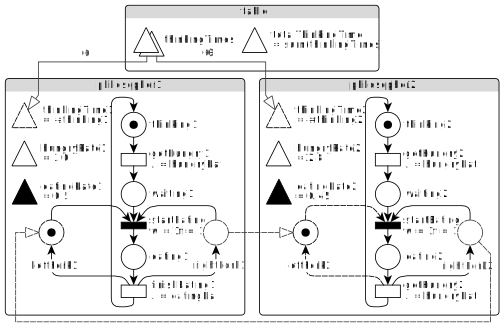
\includegraphics[scale=0.9]{figures/rgspn_example}
  \caption{Example \textabbr{RGSPN} model with an aggregate performance measure.}
  \label{fig:rgspn:example}
\end{figure}

\begin{runningExample}
  \label{ex:rgspn:example}
  \Vref{fig:rgspn:example} shows an \textabbr{RGSPN} model of the dining philosophers problem with two philosophers sitting around a table.

  While the immediate transitions \symb{start\-Eating1} and \symb{start\-Eating2} have constant weights and priorities, the timed transitions all refer to different symbols in their rate expressions. Node the difference between the variables \symb{hungry\-Rate1}, \symb{hungry\-Rate2} and the parameters \symb{eating\-Rate1}, \symb{eating\-Rate2}. Although these variables and symbols are all set to real number constants, the parameters are preserved as continuously changeable quantities when the model is passed to an external tool.

  The self-contained subnets \symb{philosohper1} and \symb{philosopher2} contain reference places \symb{right\-Fork1} and \symb{right\-Fork2}. The subnets are connected by reference assignments. The reference places specify no initial marking at all---not even a zero marking---, because they are slaves of the pointed master symbols \symb{left\-Fork2} and \symb{left\-Fork1}, respectively.

  The performance measures \symb{thinking\-Time1} and \symb{thinking\-Time2} are added to the collection \symb{thinking\-Times}. Thus the aggregate performance measure \symb{total\-Thinking\-Time} can be formed by the aggregation operator \lit{sum}.
\end{runningExample}

\subsection{Type system}
\label{ssec:rgspn:typesystem}

Type systems are tractable syntactic methods for proving the absence of certain unwanted behaviors by classifying terms according to the values they compute~\citep[Chapter~1]{Pierce02tapl}. On the other hand, static type systems for symbols in a modular Petri net were introduced by \citet{Kindler07modular}. In \textAbbr{RGSPN}s, types are used in both senses for classifying expressions, which are terms describing the quantitative aspects of the stochastic model, as well as symbols, which carry structural information.

The main unwanted behavior is the dependence of some expression on contextual information that is not available when the expression is evaluated. For example, the inscription of a Petri net arc should not depend on the state space of the Petri net, as the inscriptions themselves determine the reachable states.

The possible types are described by the following \textabbr{EBNF}-like grammar:
\begin{equation}
  \begin{aligned}
    \ebnfVar{Type} &\ebnfEq \lit{place} \mid \lit{tran} \mid \ebnfVar{VarType} \mid \bagtype{\ebnfVar{Type}} \text, \\
    \ebnfVar{VarType} &\ebnfEq \vartype{\ebnfVar{Dependence}}{\ebnfVar{Pretype}} \text,\\
    \rel{Dependence} &\ebnfEq \lit{const} \mid \lit{param} \mid \lit{marking} \mid \lit{weight} \mid \lit{prop} \mid \lit{path} \text, \\
    \ebnfVar{Pretype} &\ebnfEq \lit{int} \mid \lit{double} \mid \lit{boolean} \text.
  \end{aligned} \label{eq:rgspn:type-ebnf}
\end{equation}

The types \lit{place} and \lit{tran} correspond to places and transitions in the \textabbr{RGSPN} and the references thereof. Types of collections are formed by appending the \emph{collection qualifier} suffix \lit{[]} to the type of the members.

The types of variables deviate from routine. Inspired by conventions from the presentation of substructural type systems (see e.g.~\cite{Walker05substructural}) the types of variables are split into a qualifier and a \emph{pretype}. The pretype part expresses the domain of values, \lit{boolean} for truth values \(\mathbb{B} = \{\lit{true}, \lit{false}\}\), \lit{int} for integers and \lit{double} for real numbers.

The \emph{dependence qualifier} specifies the evaluation context of an expression as follows:
\begin{compactitem}
\item A \lit{const} expression yields a value without further input.
\item A \lit{param} expression refers to the values of continuous model parameters, which are embodied by parameter symbols.
\item A \lit{marking} expression refers to the token counts of places; therefore it yields a different value in different Petri net markings.
\item A \lit{weight} expression is both parameter- and marking-dependent.
\item A \lit{prop} expression is a performance measure or query that can be determined by model checking and stochastic analysis, but may also depend on the initial marking.
\item A \lit{path} expression is a path property defined along a trace of model execution. It may be a complete \textabbr{LTL} query or appear as a path formula in a \(\textabbr{CTL}^*\) \lit{prop} query.
\end{compactitem}

Because symbol kinds are separated from types, the type system can be adapted for many different scenarios while leaving the Petri net structure intact. Some of these possible extension based on existing literature are explored in Remarks~\ref{rem:rgspn:parametric} and \ref{rem:rgspn:colored}.

\begin{remark}\label{rem:rgspn:parametric}
  Some analysis methods only allow specific kinds of parameter-dependence, such as \(C^1\) differentiable expressions~\citep{Blake88sensitivity} or rational functions~\citep{Hahn11parametric}. However, no attempt is make to track different classes of parameter-dependent functions in \lit{param} expressions, because the restrictions on parametric expressions are highly specific to these analysis methods. If such validations is required, either the \textabbr{RGSPN} can be inspected when being exported for analysis, or the type system can be modified for the needs of the particular analysis method.
\end{remark}

\subsubsection{Subtyping}

The type system proposed in \cref{eq:rgspn:type-ebnf} can be overly rigid, because otherwise valid usages of expressions are forbidden, e.g.~a \lit{const} literal is incompatible with a \lit{marking} context. We introduce subtyping to our type system for flexibility by enabling coercions between different dependence contexts and pretypes.

Subtyping is a binary relation \({\subtype} \subseteq \rel{Type} \times \rel{Type}\), where \(\tau \subtype \tau'\) signifies that terms of type \(\tau\) are convertible to type \(\tau\). It is reflexive, i.e.~\(\tau \subtype \tau\) for all \(\tau \in \rel{Type}\).

Subtyping for variable types is the direct product of the partial orders
\begin{equation}\label{eq:rgspn:partial-order}
  \mleft(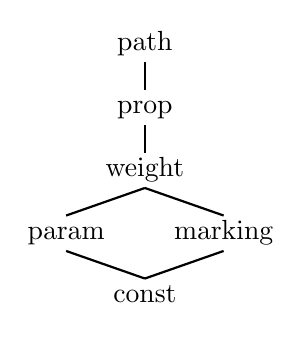
\begin{tikzpicture}[x=1cm,y=0.8cm,inner sep=0pt,thick,baseline=(weight.base)]
    \node (const) at (0, 0) {\strut\lit{const}};
    \node (param) at (-1,1) {\strut\lit{param}};
    \node (marking) at (1,1) {\strut\lit{marking}};
    \node (weight) at (0,2) {\strut\lit{weight}};
    \node (prop) at (0,3) {\strut\lit{prop}};
    \node (path) at (0,4) {\strut\lit{path}};
    \draw (const.north) -- (param.south);
    \draw (const.north) -- (marking.south);
    \draw (param.north) -- (weight.south);
    \draw (marking.north) -- (weight.south);
    \draw (weight) -- (prop);
    \draw (prop) -- (path);
  \end{tikzpicture}\mright) \mkern10mu\times\mkern10mu
  \mleft(\;\begin{tikzpicture}[x=1.5cm,y=1.2cm,inner sep=0pt,thick,baseline=($(int.base)!0.5!(double.base)$)]
    \node (int) at (0, 0) {\strut\lit{int}};
    \node (double) at (0,1) {\strut\lit{double}};
    \node (boolean) at (-1,0) {\strut\lit{boolean}};
    \draw (int) -- (double);
  \end{tikzpicture}\;\mright)
\end{equation}
of the sets \rel{Dependence} and \rel{Pretype}, respectively, where comparable elements are connected with upward paths in the style of e.g.~\citet{Walker05substructural}. For example, \(\vartype{\lit {const}}{\lit{int}} \subtype \vartype{\lit{marking}}{\lit{double}}\), because \(\lit{const} \preceq \lit{marking}\) and \(\lit{int} \preceq \lit{double}\) in the partial orders. The semantics of variable type coercions are discussed in \vref{ssec:rgspn:semantics}.

Collection types are covariant in their member types; therefore \(\tau \subtype \tau'\) if and only if \(\bagtype{\tau} \subtype \bagtype{\tau'}\). Type coercion of collections is performed elementwise.

\begin{remark}\label{rem:rgspn:colored}
  It would be possible to include more elaborate abstract syntax and subtyping rules for types, for example to describe colored Petri nets, where scalar token counts in markings are replaced by multisets over the elements of the \emph{color class} or \emph{sort} corresponding to each place. In the colored setting, instead of a single \lit{place} type, types of places carry a sort parameter. \citet{Kindler07modular} studied modular colored Petri nets with sort and operator symbols. A sort symbol reference is a color class that can be imported into the module from outside and is thus left abstract inside the module. Types of places thus may depend on the sort symbols.

  Modular colored nets may also contain \emph{operator} symbols, which transform members of a color class into another. In our framework, these could be modeled by symbols of type \(\tau \to \sigma\), i.e.~operators that transform values of type \(\tau\) into values of type \(\sigma\), extending syntax of types~\(\ebnfVar{Type} \ebnfEq \ldots \mid \ebnfVar{Type} \to \ebnfVar{Type}\). The arising challenges seem to require more elaborate type theoretical machinery, such as typed lambda calculus with subtyping (see e.g. Chapters~15 and~16 of~\cite{Pierce02tapl}).
\end{remark}

\subsection{Formal definition}

In this section we first define \textabbr{RGSPN} signatures as set of symbols of various kinds.\todo{Change \emph{kinds}.} Then the definition of an \textabbr{RGSPN} on a given signature is elaborated, which extends the signature with the properties of the symbols and the edges of the net. This separation allows deferring the details of the \emph{expressions} of a signature to \vref{sec:rgspn:expression} even though expression will serves as the properties of symbols in the definition of \textAbbr{RGSPN}s.

\begin{dfn}\label{dfn:rgspn:rgspn}
  An \emph{\textabbr{RGSPN} signatrue} is a 12-tuple
  \begin{equation}
    \Sigma = \ltup P, T_T, T_i, V, \Par, R, C, \rel{dep}, \rel{pretype}, \rel{value}, \rel{target}, \rel{member}\rtup \text,
  \end{equation}
  where the sets \(P, T_t, T_i, V, \Par, R, C,\) are disjoint and
  \begin{compactitem}
  \item \(P\) is a set of \emph{places};
  \item \(T_T\) and \(T_i\) are a sets of \emph{timed} and \emph{immediate transitions}, respectively;
  \item \(V\) is a set of \emph{variables};
  \item \(\Par\) is a set of \emph{parameters};
  \item \(R\) is a set of \emph{references};
  \item \(C\) is a set of \emph{collections};
  \item \(\rel{dep}\colon V \to \rel{Dependence}\) is the \emph{variable dependence} function;
  \item \(\rel{pretype}\colon V \to \rel{Pretype}\) is the \emph{variable pretype} function;
  \item \(\rel{value}\colon V \cup \Par \to \Expr_\Sigma \cup \mathbb{R}\) is a function, such that \(\rel{value}(v) \in \Expr_\Sigma\) for all \(v \in V\) and \(\rel{value}(\theta) \in \mathbb{R}\) for all \(\theta \in \Par\);
  \item \(\rel{target}\colon R \to \rel{Type}\) is the \emph{reference target type} function;
  \item \(\rel{member}\colon C \to \rel{Type}\) is the \emph{collection member type} function.
  \end{compactitem}
\end{dfn}

We will abuse notation such that \(\Sigma\) also stands for the set \(P \cup T_t \cup T_i \cup V \cup \Par \cup R \cup C\) of all symbols. Furthermore, \(\Expr_\Sigma\) will denote the set of all algebraic expressions that may mention symbols of \(\Sigma\).

\begin{dfn}
  An \emph{\textabbr{RGSPN}} is a 10-tuple \(N = \ltup \Sigma, m_0, \lambda, w, \pi, {\outarc}, {\inarc}, {\inharc}, {\assign}, {\member} \rtup\), where
  \begin{compactitem}
  \item \(\Sigma = \ltup P, T_T, T_i, V, \Par, R, C, \ldots\rtup\) is an \textabbr{RGSPN} signature;
  \item \(m_0 \colon P \to \Expr_\Sigma\) is the \emph{initial marking} function;
  \item \(\lambda \colon T_T \to \Expr_\Sigma\) is the \emph{timed transition rate} function;
  \item \(w\colon T_i \to \Expr_\Sigma\) is the \emph{immediate transition weight} function;
  \item \(\pi\colon T_i \to \Expr_\Sigma\) is the \emph{immediate transition priority} function;
  \item \({\outarc}, {\inarc}, {\inharc} \subseteq \Sigma \times \Expr_\Sigma \times \Sigma\) are the relations of \emph{output, input} and \emph{inhibitor arcs}, respectively, which are free of parallel arcs, i.e.~\(\ltup p, e_1, t \rtup, \ltup p, e_2, t \rtup \in {\outarc}\) implies \(e_1 = e_2\) and this property holds also for \(\inarc\) and \(\inharc\);
  \item \({\assign} \subseteq R \times \Sigma\) is the relation of \emph{reference assignments};
  \item \({\member} \in \rel{Multiset}(\Sigma \times \Sigma)\) is the multiset relation of \emph{collection memberships}.
  \end{compactitem}
\end{dfn}

Note the separation between timed \(T_T\) and immediate transitions \(T_i\). In \textAbbr{GSPN}s timed and immediate transitions are usually discriminated by setting \(\pi(t) = 0\) for all \(t \in T_T\)~\citep{Marsan84gspn}. However, in our setting the priority \(\pi(t)\) may contain an algebraic expression; therefore determining whether \(\pi(t) = 0\) would require nontrivial computations. By explicitly partitioning the set of transitions \(T = T_T \djcup T_i\) this computation is avoided.
 
All quantitative aspects of the net are described by expressions \(\Expr_\Sigma\) with the exception of the values of the parameters, which must be real numbers.\todo{Should this go somewhere else?} As any computation is forbidden inside parameter values, so that parameter synthesis tool may set new values of the parameters without needing to respect any constraints between parameter values implicit in the value computations. Explicit constraints, such as interval bounds for parameters may be added as an extension of \textAbbr{RGSPN}s; however, they are currently not supported. If multiple values depending on a shared set of parameters are needed, variable symbols with value expressions may be used instead.

Edges of the net are between pairs of arbitrary symbols, e.g.~arcs are not restricted to go from place symbols to transition symbols, because any symbol may be replaced by a reference of compatible type. However, reference assignments must assign the symbol to be pointed at to a reference, as no other symbol kind can act as an assignable.

Although parallel arcs are forbidden, parallel collection membership edges are permitted by making \({\member}\) a multiset relation, i.e.~a \emph{bag} of tuples, such as \(\Lbag \ltup c, s \rtup, \ltup c, s \rtup, \ldots \Rbag\).

We will write \(p \overset{e}{\outarc} t\), \(p \overset{e}{\inarc} t\), \(p \overset{e}{\inharc} t\), \(r \assign s\) and \(c \member s\) for \(\ltup p, e, t \rtup \in {\outarc}\), \(\ltup p, e, t \rtup \in {\inarc}\), \(\ltup p, e, t \rtup \in {\inharc}\), \(\ltup r, s \rtup \in {\assign}\) and \(\ltup c, s \rtup \in {\member}\), respectively.

\subsubsection{Type checking}

Types for the symbols of the net are synthesized by the function \(\rel{type}\colon \Sigma \to \rel{Type}\) defined as
\begin{equation}
  \rel{type}(s) = \left\{\begin{array}{@{}l@{\quad}l@{\qquad}l@{\quad}l@{}}
    \lit{place} \text, & \text{if \(s \in P\),}
    & \lit{tran} \text, & \text{if \(s \in T\),} \\
    \vartype{\rel{dep}(s)}{\rel{pretype}(s)} \text, & \text{if \(s \in V\),}
    & \vartype{\lit{param}}{\lit{double}} \text, & \text{if \(s \in \Par\),} \\
    \rel{target}(s) \text, & \text{if \(s \in R\),}
    & \bagtype{\rel{member}(s)} \text, & \text{if \(s \in C\),}
  \end{array}\right.
\end{equation}
The types of places and transitions match their kinds, while variables have a variable type according to their dependence and pretype. The types of parameters are fixed to \(\vartype{\lit{param}}{\lit{double}}\), as they are continuous and parameter dependent by definition. References always have the type of the symbol they may point at; therefore they may stand for the pointed symbol. Collections append a collection type qualifier to the type of their members.

The \emph{typing relation} \({\_} \vdash {\_} \oftype {\_}\) assigns types to expressions \(e \in \Expr_\Sigma\). We write \(\Sigma \vdash e \oftype \tau\) if \(e\) is of type \(\tau\) in the context of the \textabbr{RGSPN} signature \(\Sigma\). As it will be seen in \vref{sec:rgspn:expression} the typing relation respects subtyping, i.e.
\begin{equation}
  \frac{\Sigma \vdash e \oftype \tau \quad \tau \subtype \tau'}{%
    \Sigma \vdash e \oftype \tau'} \Tag{T-Sub} \,\text.
\end{equation}

In well-typed \textAbbr{RGSPN}s, where expressions and edges respect strong typing to ensure context-appropriate use of symbols and expressions within both the structural part of the net and its queries. Below we propose some typing requirements that make analysis tractable without greatly restricting the modeler.

\todo{Should we split the formal stuff and the discussion?}
\begin{dfn}
  An \textabbr{RGSPN} is well-typed if it has the following properties:
  \begin{compactitem}
  \item For all \(p \in P\) the initial marking is an integer constant, \(\Sigma \vdash m_0(p) \oftype \vartype{\lit{const}}{\lit{int}}\).
  \item For all timed transitions \(t \in T_T\) the transition rate is a possibly marking- and parameter-dependent real number, \(\Sigma \vdash \lambda(t) \oftype \vartype{\lit{weight}}{\lit{double}}\).
  \item For all immediate transitions \(t \in T_i\) the probability weight is a possibly marking- and parameter-dependent real number, \(\Sigma \vdash w(t) \oftype \vartype{\lit{weight}}{\lit{double}}\). The transition priority is typed much more conservatively by requiring an integer constant, such that \(\Sigma \vdash \pi(t) \oftype \vartype{\lit{const}}{\lit{int}}\) holds.
  \item For all variables \(v \in V\) the value expression must match the type of the variable, \(\Sigma \vdash \rel{value}(v) \oftype \rel{type}(v)\).
  \item All arcs \(p \overset{e}{\outarc} t\), \(p \overset{e}{\inarc} t\) or \(p \overset{e}{\inharc} t\) go between places and transitions such that \(\rel{type}(p) \subtype \lit{place}\) and \(\rel{type}(t) \subtype \lit{tran}\) holds. The inscription \(e\) may depend on the marking, \(\Sigma \vdash e \oftype \vartype{\lit{marking}}{\lit{int}}\),
  \item For all \(r \assign s\), \(s\) is a compatible target of \(r\), \(\rel{type}(s) \subtype \rel{target}(r)\).
  \item For all \(c \member s\), \(s\) is a valid member of \(c\), \(\rel{type}(s) \subtype \rel{member}(s)\).
  \end{compactitem}
\end{dfn}

\begin{remark}
  The requirements are based on the assumptions in \textabbr{GSPN} and \textabbr{CTMC} solution algorithms. While the inscriptions of arcs \(e\) are allowed to have dependence \lit{marking}, because marking-dependent arcs may lead to simplifications of stochastic models~\citep{Ciardo93decomposition}. However, as some external tools only support arcs with constant inscriptions, \(\Sigma \vdash e \oftype \vartype{\lit{const}}{\lit{int}}\) may be enforced instead for compatibility.

  Similarly, marking-dependent immediate transition weight can also pose a difficulty in solving the model~\citep{Teruel03netlevel}, which can be averted by requiring \(\Sigma \vdash w(t) \oftype \vartype{\lit{param}}{\lit{double}}\) for all \(t \in T_i\). In contrast, some state-space explorations methods, such as the decision diagram based algorithm proposed by~\citet{Marussy17priorities}, may permit marking-dependent priorities \(\Sigma \vdash \pi(t) \oftype \vartype{\lit{marking}}{\lit{int}}\).
\end{remark}
  
From now on all discussed \textAbbr{RGSPN}s will be assumed to be well-typed.

\begin{figure}
  \centering
  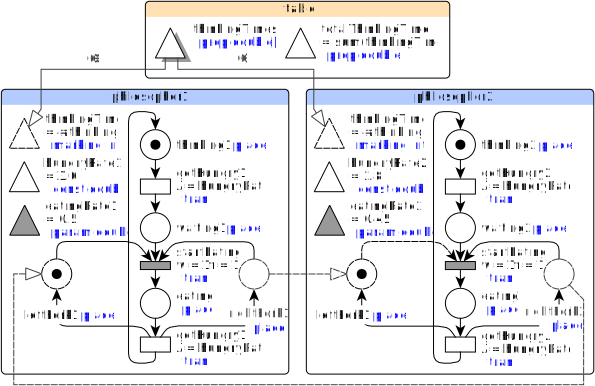
\includegraphics[scale=0.9]{figures/rgspn_example_typed}
  \caption{Example \textabbr{RGSPN} with type annotations.}
  \label{fig:rgspn:example-typed}
\end{figure}

\begin{runningExample}
  \Vref{fig:rgspn:example-typed} shows the model from \vref{ex:rgspn:example} extended with type annotations in blue. Places, transitions and parameters have their expected types \lit{place}, \lit{tran}, \(\vartype{\lit{param}}{\lit{double}}\). Variables are annotated according to their \rel{dep} and \rel{pretype}, while collections bear the collection qualifier suffix \lit{[]}.

  There are several examples of subtyping in action: the symbols \symb{thinking\-Time1}, \symb{thinking\-Time2}, \symb{eating\-Rate1}, \symb{eating\-Rate2} are used as rates of timed transitions despite their types \(\vartype{\lit{const}}{\lit{double}}\) and \(\vartype{\lit{param}}{\lit{double}}\). The collection \symb{thinking\-Times} of \(\vartype{\lit{prop}}{\lit{double}}\) members contains the symbols \symb{thinking\-Time1} and \symb{thinking\-Time2} of type \(\vartype{\lit{marking}}{\lit{int}}\).
\end{runningExample}

\section{Expressions}
\label{sec:rgspn:expression}

In this section we propose an abstract syntax for expressions that describe the quantitative aspects of \textabbr{RGSPN} models, including arc inscriptions, initial markings firing policies in \vref{dfn:rgspn:rgspn}, as well as the performance measures and queries of interest.

The expression language \(\textabbr{CTL}^*\) includes state and path operators in addition to references to net elements, basic arithmetic and logical operators. These additional operators enable defining queries concerning \textabbr{CTL}, \textabbr{LTL} or \(\textabbr{CTL}^*\) properties. Similarly to the flexibility of the type system, the syntax of expressions can be also extended if the definition of further properties, such as \textabbr{CSL} formulas are desired. Validation and interpretation of the queries, such as checking whether a \(\textabbr{CTL}^*\) formula is in \textabbr{CTL} when full \(\textabbr{CTL}^*\) is not supported, is the responsibility of the external model checking tool.

The valid expression on an \textabbr{RGSPN} signature \(\Sigma\) form the set \(\Expr_\Sigma\) described by the following \textabbr{EBNF}-like grammar:
\begin{equation}
  \label{eq:rgspn:expression}
  \begin{aligned}
    \ebnfV{\Expr_\Sigma} &\ebnfEq \ebnfVar{Literal} 
    \mid \ebnfV{\Sigma} \mid \lit\# \ebnfV{\Sigma} \mid \ebnfVar{Aggregate} \lit( \ebnfV{\Sigma} \lit)
    \mid \ebnfVar{Unary}\; \ebnfV{\Expr_\Sigma} \\*
    &\ebnfCont \ebnfV{\Expr_\Sigma} \mathbin{\ebnfVar{Binary}} \ebnfV{\Expr_\Sigma}
    \mid \lit{if}\ \lit(\ebnfV{\Expr_\Sigma}\lit)\ \ebnfV{\Expr_\Sigma}\ \lit{else}\ \ebnfV{\Expr_\Sigma} \text, \\
    \ebnfVar{Literal} &\ebnfEq \ebnfV{\NN} \mid \ebnfV{\RR} \mid \ebnfV{\BB} \text, \\
    \ebnfVar{Aggregate} &\ebnfEq \lit{sum} \mid \lit{prod}
    \mid \lit{all} \mid \lit{any} \text, \\  
    \ebnfVar{Unary} &\ebnfEq \lit{+} \mid \lit{-} \mid \lit{!} \mid \lit{A} \mid \lit{E} \mid \lit{X}  \mid \lit{F} \mid \lit{G} \text, \\
    \ebnfVar{Binary} &\ebnfEq \lit{+} \mid \lit{-} \mid \lit{*} \mid \lit{/}
    \mid \lit{==} \mid \lit{!=} \mid \lit{<} \mid \lit{<=} \mid \lit{>} \mid \lit{>=}
    \mid \lit{\&\&} \mid \lit{||} \mid \lit{U} \text.
  \end{aligned}
\end{equation}

The expression language contains Boolean, integer and real literals, a standard set of unary and binary operators, a ternary conditional operator, as well as \(\textabbr{CTL}^*\) state operators \lit{A}, \lit{E} and path operators \lit{X}, \lit{F}, \lit{G}, \lit{U}. Variable symbols and references thereof from \(\Sigma\) may be mentioned as-is and are interpreted as the \rel{value}s of the variables. Places can be also mentioned by prefixing them with \lit{\#} and correspond to \lit{marking} dependent expressions referring to the number of tokens on the place. Collections must be paired with an \emph{aggregation operator} to turn their multiset of member symbols into a single value.

Note that marking expressions and collection aggregations directly take a symbol from \(\Sigma\) instead of an expression \(\Expr_\Sigma\); therefore \enquote{\(\lit{if}\ \lit(\lit\#p_1 > 0\lit)\ \lit\#p_2\ \lit{else}\ \lit\#p_3\)} is a valid expression, but \enquote{\(\lit\#\lit(\lit{if}\ \lit(\lit\#p_1 > 0\lit)\ p_2\ \lit{else}\ p_3\lit)\)} is invalid. This restriction, while not constraining expressivity significantly, allow for more straightforward inlining and implification of expressions when the \textabbr{RGSPN} is transformed into a \textabbr{GSPN}.

\subsection{Typing}

\begin{table}
  \caption{Typing rules for expressions.}
  \label{fig:rgspn:typing}
  \begin{tabu}{@{}X[c]r@{}}
    \toprule
    \(\dfrac{{\diamond} \in \{\lit{+}, \lit{-}\}
      \quad \rho \in \{\lit{int}, \lit{double}\}
      \quad \Sigma \vdash e \oftype \delta\,\rho
    }{\Sigma \vdash \mathop{\diamond} e \oftype \delta\,\rho}\),
    & \Tagstyle{T-Unary\(\pm\)} \\[1.2ex]
    \(\dfrac{\Sigma \vdash e \oftype \delta\,\lit{boolean}
    }{\Sigma \vdash \lit{!} e \oftype \delta\,\lit{boolean}}\),
    & \Tagstyle{T-UnaryNot} \\[1.2ex]
    \(\dfrac{{\diamond} \in \{\lit{A}, \lit{U}\}
      \quad \Sigma \vdash e \oftype \vartype{\lit{path}}{\lit{boolean}}
    }{\Sigma \vdash \mathop{\diamond} e \oftype \vartype{\lit{prop}}{\lit{boolean}}}\),
    & \Tagstyle{T-UnaryState} \\[1.2ex]
    \(\dfrac{{\diamond} \in \{\lit{X}, \lit{F}, \lit{G}\}
      \quad \Sigma \vdash e \oftype \vartype{\lit{path}}{\lit{boolean}}
    }{\Sigma \vdash \mathop{\diamond} e \oftype \vartype{\lit{path}}{\lit{boolean}}}\),
    & \Tagstyle{T-UnaryPath} \\[1.2ex]
    \(\dfrac{{\diamond} \in \{\lit{+}, \lit{-}, \lit{*}\}
      \quad \rho \in \{\lit{int}, \lit{double}\}
      \quad \Sigma \vdash e_1 \oftype \delta\,\rho
      \quad \Sigma \vdash e_2 \oftype \delta\,\rho
    }{\Sigma \vdash e_1 \mathbin{\diamond} e_2 \oftype \delta \,\rho}\),
    & \Tagstyle{T-BinNumeric} \\[1.2ex]
    \(\dfrac{\Sigma \vdash e_1 \oftype \delta\,\lit{double}
      \quad \Sigma \vdash e_2 \oftype \delta\,\lit{double}
    }{\Sigma \vdash e_1 \mathbin{\lit/} e_2 \oftype \delta \,\lit{double}}\),
    & \Tagstyle{T-BinDiv} \\[1.2ex]
    \(\dfrac{\Sigma \vdash e_1 \oftype \vartype{\lit{path}}{\lit{boolean}}
      \quad \Sigma \vdash e_2 \oftype \vartype{\lit{path}}{\lit{boolean}}
    }{\Sigma \vdash e_1 \mathbin{\lit{U}} e_2 \oftype \vartype{\lit{path}}{\lit{boolean}}}\),
    & \Tagstyle{T-BinUntil} \\[1.2ex]
    \(\dfrac{{\diamond} \in \{\lit{==}, \lit{!=}\}
      \quad \Sigma \vdash e_1 \oftype \delta\,\rho
      \quad \Sigma \vdash e_2 \oftype \delta\,\rho
    }{\Sigma \vdash e_1 \mathbin{\diamond} e_2 \oftype \delta\,\lit{boolean}}\),
    & \Tagstyle{T-BinEq} \\[1.2ex]
    \(\dfrac{{\diamond} \in \{\lit{<}, \lit{<=}, \lit{>}, \lit{>=}\}
      \quad \Sigma \vdash e_1 \oftype \delta\,\lit{double}
      \quad \Sigma \vdash e_2 \oftype \delta\,\lit{double}
    }{\Sigma \vdash e_1 \mathbin{\diamond} e_2 \oftype \delta\,\lit{boolean}}\),
    & \Tagstyle{T-BinCompare} \\[1.2ex]
    \(\dfrac{{\diamond} \in \{\lit{\&\&}, \lit{||}\}
      \quad \Sigma \vdash e_1 \oftype \delta\,\lit{boolean}
      \quad \Sigma \vdash e_2 \oftype \delta\,\lit{boolean}
    }{\Sigma \vdash e_1 \mathbin{\diamond} e_2 \oftype \delta\,\lit{boolean}}\),
    & \Tagstyle{T-BinLogical} \\[1.2ex]
    \(\dfrac{\Sigma \vdash e_1 \oftype \delta\,\lit{boolean}
      \quad \Sigma \vdash e_2 \oftype \delta\,\rho
      \quad \Sigma \vdash e_3 \oftype \delta\,\rho
    }{\Sigma \vdash \lit{if}\ \lit(e_1\lit)\ e_2\ \lit{else}\ e_3 \oftype \delta\,\rho}\), &
    \Tagstyle{T-If} \\[1.2ex]
    \(\dfrac{\rel{agg} \in \{\lit{sum}\mkern1mu, \lit{prod}\}
      \quad \rho \in \{\lit{int}, \lit{double}\}
      \quad \rel{type}(b) = \bagtype{\delta\,\rho}
    }{\Sigma \vdash \rel{agg}\lit(b\lit) \oftype \delta\,\rho}\),
    & \Tagstyle{T-AggNumeric} \\[1.2ex]
    \(\dfrac{\rel{agg} \in \{\lit{all}, \lit{any}\}
      \quad \rel{type}(b) = \bagtype{\delta\,\lit{boolean}}
    }{\Sigma \vdash \rel{agg}\lit(b\lit) \oftype \delta\,\lit{boolean}}\),
    & \Tagstyle{T-AggLogical} \\[1.2ex]
    \multicolumn{2}{@{}p{\linewidth}@{}}{
      \begin{tabu}{@{}X[c]rX[c]r@{}}
        \(v \oftype \rel{type}(v)\),
        & \Tagstyle{T-Var}
        & \(\dfrac{\rel{type}(p) \subtype \lit{place}
        }{\lit{\#} p \oftype \vartype{\lit{marking}}{\lit{int}}}\),
        & \Tagstyle{T-Marking} \\[1.2ex]
        \(\dfrac{\ell \in \llbracket\rho\rrbracket
        }{\Sigma \vdash \ell \oftype \lit{const}\,\rho}\),
        & \Tagstyle{T-Literal}
        & \(\dfrac{\Sigma \vdash e \oftype \tau\quad \tau \subtype \tau'
        }{\Sigma \vdash e \oftype \tau'}\),
        & \Tagstyle{T-Sub}
      \end{tabu}
    } \\
    \multicolumn{2}{@{}l@{}}{
      \small where \(\llbracket\lit{int}\rrbracket = \mathbb{N}\),
      \(\llbracket\lit{double}\rrbracket = \mathbb{Z}\) and
      \(\llbracket\lit{boolean}\rrbracket = \mathbb{B}\).
    } \\
    \bottomrule
  \end{tabu}
\end{table}

A complete set of typing rules for \(\Expr_\Sigma\) is presented in~\vref{fig:rgspn:typing}, which described the relation \(\_ \vdash \_ \oftype \_\). The judgement \(\Sigma \vdash e \oftype \tau\) assigns a type \(\tau\) to an expression \(e \in \rel{Expr}(\Sigma)\) in the context of an \textabbr{RGSPN} signature \(\Sigma\). 

The types of unary operators, binary operators, conditional and aggregate expressions are captured by the rules \textsc{T-Unary}, \textsc{T-Bin}, \textsc{T-If} and \textsc{T-Agg}. Instead of introducing types for operators and typing rules for operator application, typing rules for all operators are written out explicitly. While this approach increases the number of typing rules considerably, the lack of function types and polymorphic types allows the syntax of \(\rel{Type}\) to remain simple. If more generality is desired, the type system may be extended to support user-defined operators and operator types as described in \vref{rem:rgspn:colored}.

In spite of being handled only in the type derivation rules, several operators are polymorphic in the types of the arguments. However, \textsc{T-BinaryDiv} forces both arguments of the division operator be be real numbers, so that ambiguities concerning integer division are avoided. Most compound expressions are \emph{dependency polymorphic}, that is, the types of their arguments may have any dependency qualifier \(\delta\), which will be inherited by the type of the whole expression. The exception are the \(\textabbr{CTL}^*\) operators, which operate on \lit{path} formulas and produce \lit{path} or \lit{prop} state formulas. 

Variable and marking references are handled by \textsc{T-Var} and \textsc{T-Marking}. Referring to markings of places always produces a \lit{marking} dependent \lit{int}. \textsc{T-Literal} assigns \lit{const} types to literal constants. Lastly, \textsc{T-Sub} allows the use of subtyping in type derivations.

\subsection{Semantics}
\label{ssec:rgspn:semantics}

In this section we sketch the semantics of \(\Expr_\Sigma\) both for structural expression of an \textabbr{RGSPN} and for performance measures and queries. Most of the expression evaluation happens in external analysis tools when marking- and parameter-dependent expressions are interpreted to construct a \textabbr{CTMC} from the Petri net and when queries are answered. Therefore, exporting \textAbbr{RGSPN}s for external tools must be performed with care to ensure that the tool interprets the provided input according to these semantics. This may require nontrivial transformation of the expressions to the input language of the tool and may even be impossible to fully achieve when the external tool is missing some analysis features. In the latter case, the user receives an error message during export.

Values of pretypes \lit{boolean}, \lit{int} and \lit{double} can be interpreted as members of the sets \(\mathbb{B} = \{\lit{true}, \lit{false}\}\) of truth values, \(\mathbb{Z}\) of integers and \(\mathbb{R}\) of real numbers, respectively.\footnote{In practice, representations on integers and floating-point numbers with a finite number of bits are used instead. However, this distinction only becomes important in the external analysis tools, where finite numerical precision necessitates careful design of algorithms to control approximation error \todo*{Cite Bayer MDP paper}.} Formally, pretypes have the interpretations
\begin{align}
  \llbracket \lit{boolean} \rrbracket &= \mathbb{B} \text,
  & \llbracket \lit{int} \rrbracket &= \mathbb{Z} \text,
  & \llbracket \lit{double} \rrbracket &= \mathbb{R} \text.
\end{align}

Variable types \(\vartype{\delta}{\rho}\) can be viewed as functions from some \emph{context} determined by the dependence qualifier \(\delta\) to the set \(\llbracket \rho \rrbracket\). In the case \(\delta = \lit{const}\), the context is empty, so \(\llbracket \vartype{\lit{const}}{\rho} \rrbracket\) is isomorphic to \(\llbracket \rho \rrbracket\). For other qualifiers, the context may be comprised of a vector \(\vec{\uptheta} \in \mathbb{R}^{\lvert \Par \rvert}\) of parameter values and the current marking of the Petri net \(m\). Queries with \lit{prop} and \lit{path} dependence may also require the entire \textabbr{CTMC} that describes the logical and stochastic behavior of the \textabbr{RGSPN} for evaluation. Finally, \lit{path} properties are evaluated on an execution path \(\Pi = m_1 \to m_2 \to \ldots\) of markings (or equivalently, \textabbr{CTMC} states). The interpretations of variable types can be summarized as
\begin{equation}
  \begin{array}{@{}r@{\,}c@{\ }c@{\ }c@{\ }c@{\,}l@{\,}c@{}}
    & \text{\footnotesize parameters} & \text{\footnotesize marking} & \text{\footnotesize \textabbr{CTMC}} & \text{\footnotesize path} & & \text{\footnotesize value} \\*
    \llbracket \vartype{\lit{const}}{\rho} \rrbracket \colon& & & & & &p \in \llbracket \rho \rrbracket \text, \\
    \llbracket \vartype{\lit{param}}{\rho} \rrbracket \colon& \vec{\uptheta} & & & & \mapsto &p \in \llbracket \rho \rrbracket \text, \\
    \llbracket \vartype{\lit{marking}}{\rho} \rrbracket \colon& & m & & & \mapsto &p \in \llbracket \rho \rrbracket \text, \\
    \llbracket \vartype{\lit{weight}}{\rho} \rrbracket \colon& \vec{\uptheta}\mathrlap, & m & & & \mapsto &p \in \llbracket \rho \rrbracket \text, \\
    \llbracket \vartype{\lit{prop}}{\rho} \rrbracket \colon& \vec{\uptheta}\mathrlap, & m\mathrlap, & \textabbr{CTMC} & & \mapsto &p \in \llbracket \rho \rrbracket \text, \\
    \llbracket \vartype{\lit{path}}{\rho} \rrbracket \colon& \vec{\uptheta}\mathrlap, & & \textabbr{CTMC}\mathrlap, & \Pi & \mapsto &p \in \llbracket \rho \rrbracket \text. \\
  \end{array}
\end{equation}

Type coercion from \lit{int} to \lit{double} act in the obvious way. Dependence coercion along the partial order from \vref{eq:rgspn:partial-order} introduces arguments to the interpretation functions that are ignored. For example, coercing \(\lit{const}\) to \(\lit{weight}\) results in a function that ignores its \(\vec{\uptheta}\) and \(m\) arguments while returning a constant value. The only non-straightforward coercion is from \lit{prop} to \lit{path}. In order to be consistent with \(\textabbr{CTL}^*\) formulas this conversion is defined such that the first marking \(m_1\) of the path \(\Pi = m_1 \to m_2 \to \ldots\) serves as the current marking argument \(m\) of the \lit{prop} computation when it is treated as a \lit{path} property.

Operators from \vref{eq:rgspn:expression} act pointwise on the interpretation functions, e.g.~to calculate \(e_1 \mathbin{\diamond} e_2\), \(e_1\) and \(e_2\) are separately evaluated in the dependence context, then the operator \(\diamond\) is applied to the resulting values.\footnote{This makes variable types with a dependence qualifier other than \lit{const} specializations of \emph{Reader} applicative functors \todo*{cite}.}

The \(\textabbr{CTL}^*\) operators, which explicitly require \lit{prop} and \lit{path} dependence contexts, are excepted from pointwise evaluation. A \lit{prop} expression is treated as a state predicate over markings \(m\) after plugging the parameter binding \(\vec{\uptheta}\) and the \textabbr{CTMC} into the interpretation function. Similarly, \lit{path} expressions are treated as predicates over paths \(\Pi\) and are composed by the operators according to \(\textabbr{CTL}^*\) semantics (see e.g.~\todo*{Cite}).

\todo*{The sections below should go to the transformation chapter.}

\section{Reference inlining}
\label{sec:rgspn:inlining}

\subsection{Handling inconsistent models}
\label{ssec:rgspn:inconsistent}


%%% Local Variables:
%%% mode: latex
%%% TeX-master: "../main"
%%% End:
